\documentclass[12pt,a4paper,portrait]{article}

\usepackage[portuguese]{babel} 	% hifenização
\usepackage[utf8]{inputenc} 	% acentos e cedilhas
\usepackage[T1]{fontenc} 		% evitar problemas com fonts
\usepackage{graphicx}
\usepackage{graphicx,wrapfig}
\usepackage{fancyhdr}
\usepackage{lastpage}
\usepackage[dvipsnames]{xcolor}
\usepackage{colortbl}
\usepackage{enumerate}			% Include the enumerate-package
\usepackage{listings}           % Include the listings-package
\usepackage{color}				% Include the color-package
\usepackage{askmaps}
\usepackage{booktabs}
\usepackage{xcolor}

\usepackage{babel}
\usepackage[font=small,labelfont=bf]{caption}

\pagestyle{fancy}
\fancyhf{}
\rhead{Engenharia Informática 2º Ano}
\lhead{ISMAT}
\rfoot{Página \thepage \hspace{1pt} de \pageref{LastPage}}

\setcounter{secnumdepth}{5}	% actualiza o contador máximo de níveis para subsections
\setcounter{tocdepth}{5}	% actualiza o contador máximo de níveis na Tabela de Conteudo

\begin{document}
	\begin{titlepage}
	\begin{center}
	
		% Upper part of the page. The '~' is needed because \\
		% only works if a paragraph has started.
		%
\includegraphics[width=0.95\textwidth]{./logo}~\\[1,5cm]
		
\includegraphics{./logo}
		% \includegraphics{logo_ismat}
		
		
		%\textsc{\LARGE Instituto Superior Manuel Teixeira Gomes }\\[1.5cm]
		
		\textsc{\Large Algoritmia e Estrutura de Dados}\\[1.5cm]
		
		% Title
		\newcommand{\HRule}{\rule{\linewidth}{0.5mm}}
		\HRule \\[0.4cm]
		{ \huge \bfseries Travel Salesman Problem \\[0.4cm] }
		
		\HRule \\[1.5cm]
		
		% discente e docente
		\noindent
		
		\begin{minipage}[t]{0.4\textwidth}
			\begin{flushleft} \large
				\emph{Discente(s):}\\
				Pedro \textsc{Roldan}\\
				Leandro \textsc{Moreira}\\
			\end{flushleft}
		\end{minipage}%
		\begin{minipage}[t]{0.4\textwidth}
			\begin{flushright} \large
				\emph{Docente:} \\
				Doutor Faroq \textsc{AlTam}
			\end{flushright}
		\end{minipage}
		
		\vfill
		
		% Bottom of the page
		{\large \today}
	
	\end{center}
\end{titlepage}
	\tableofcontents
	
	\lstdefinestyle{customc}{
	  belowcaptionskip=1\baselineskip,
	  breaklines=true,
	  frame=L,
	  xleftmargin=\parindent,
	  language=C,
	  showstringspaces=false,
	  basicstyle=\footnotesize\ttfamily,
	  keywordstyle=\bfseries\color{green!40!black},
	  commentstyle=\itshape\color{purple!40!black},
	  identifierstyle=\color{blue},
	  stringstyle=\color{orange},
      tabsize=1,
	}
	
	\newpage
	\section{Introdução}
		O travel salesman problem (TSP) é um problema bastante comum largamente encontrado em diversas aplicações tais como: empresas de transporte (e.g. UPS), escalas de tripulação de companhias aéreas, etc.\\
		Em principio, um vendedor necessita de efetuar uma viagem por diversas cidades, onde inicia a viagem numa determinada cidade (Casa), visita todas as cidades para vender os seus produtos, e retorna a casa.\\
		\subsection{Requisitos Minimos}	
			O TSP pode ser representado por uma lista de nós, sendo o objectivo descobrir uma serie de caminhos (Edges) entre cada um dos nós.\\\\
			Sendo que:\\
			\begin{itemize}
				\item Cada nó (Cidade) pode ser visitado apenas 1 vez.
				\item Os caminhos formam uma Tour.
				\item O custo da Tour deve ser o minimo possivel.
			\end{itemize}
			A tour TSP é um grafico direcionado, onde cada nó representa uma cidade, e cada edge representa um caminho entre 2 cidades.\\
			Cada edge têm um peso, que é no seu caso mais simples a distancia euclidiana entre os seus nós.\\
			Este peso pode ser composto por diversos fatores, no entanto neste projeto apenas se considera a distancia entre nós.\\ 			

			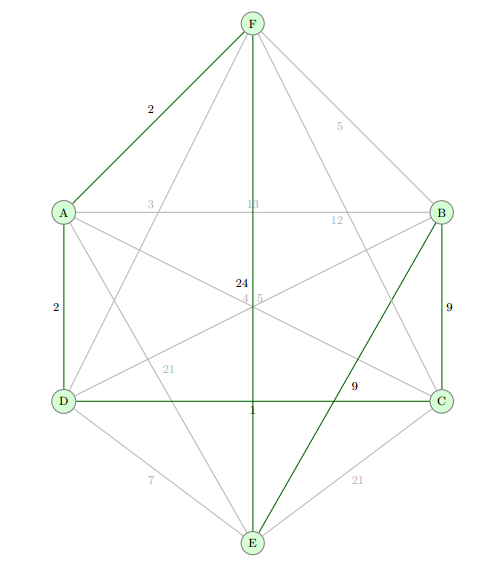
\includegraphics[width=1.0\textwidth]{imagens/1}
			\newpage
			\subsubsection{RGB Decoder} \label{ssec:num1}
				A função deste circuito é a de ao receber a indicação de posição através do grupo binário de S0 e S1, efetuar a correspondência de cor para a saída do led correspondente, através da separação do grupo de 3 bits.\\
				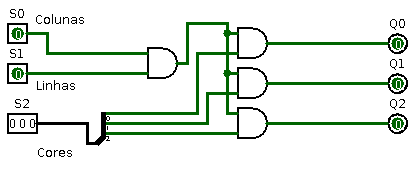
\includegraphics[width=1.0\textwidth]{imagens/rgbdec}
				\captionof{figure}{RGB Decoder}
				S0-S3: Conjunto binário de 4 bits correspondendo ao seu valor decimal\\
		\newpage						

			A ROM (read-only memory), é um tipo de memória que permite apenas a leitura, ou seja, as suas informações são gravadas uma única vez e após isso não podem ser alteradas ou apagadas, somente acedidas. São memórias cujo conteúdo é gravado permanentemente.\\\\
			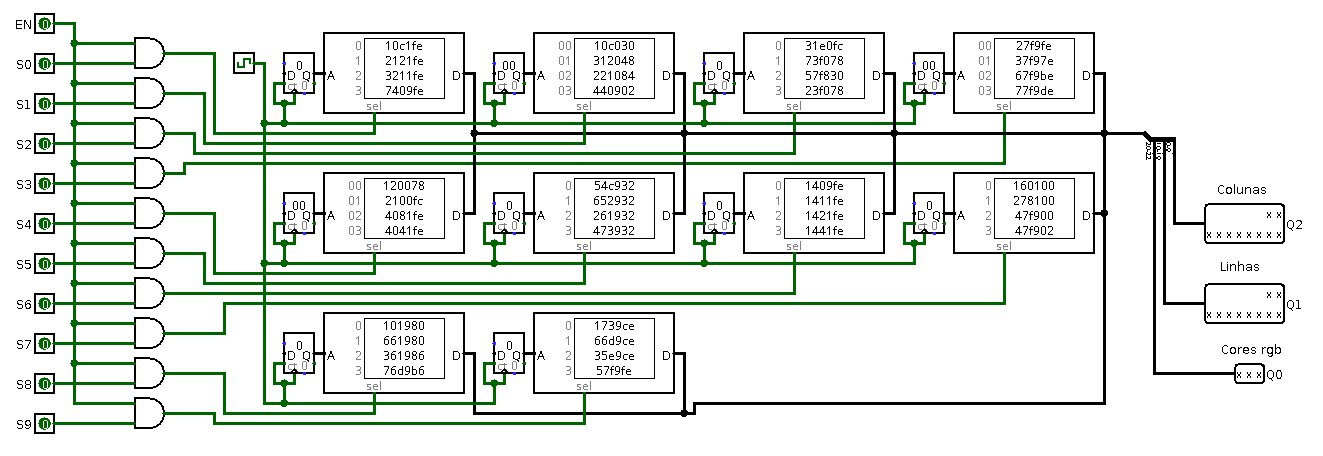
\includegraphics[width=1.0\textwidth]{imagens/romr1}
			\captionof{figure}{Circuito de controle de ROMS}
			EN: Bit de controlo de enable/disable\\
			S0-S9: Bit de entrada para seleção de ROM\\
			Q0: Conjunto de 3 bits para seleção de cor RGB\\
			Cada ROM é controlada por um contador exclusivo e um clock partilhado.\\
			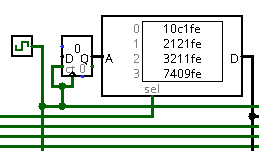
\includegraphics[width=0.5\textwidth]{imagens/rom1}
			\captionof{figure}{ROM Individual}
			Cada ROM tem uma estrutura dimensionada para cada conjunto de sequencias ..\\
			A ROM é controlada por um contador associado a um clock, que permite que, em cada ciclo o contador avançe para uma nova posição (index) da ROM e efetue a leitura da sequencia de bits armazenada, que por sua vez define o endereço do led na matriz, assim como a sua cor e estado.\\
			\subsubsection{BCD - Binary Coded Decimal} \label{sssec:bcd}
				O \cite{Garroz}\textbf{código BCD} foi criado para codificar os números decimais de 0 a 9, com 4 bits para cada dígito, ou seja, o BCD é a conversão dos decimais em um número binário de 4 bits e representa-se da seguinte forma:
				\begin{table}[!h]
					\centering
					\caption{Tabela BCD}
					\label{my-label}
					\resizebox{0.5\textwidth}{!}{%
						\begin{tabular}{@{}|l|l|@{}}
							\toprule
							\rowcolor[HTML]{BBDAFF} 
							Digito Decimal & Codigo BCD \\ \midrule
							0 & 0000 \\ \midrule
							1 & 0001 \\ \midrule
							2 & 0010 \\ \midrule
							3 & 0011 \\ \midrule
							4 & 0100 \\ \midrule
							5 & 0101 \\ \midrule
							6 & 0110 \\ \midrule
							7 & 0111 \\ \midrule
							8 & 1000 \\ \midrule
							9 & 1001 \\ \bottomrule
						\end{tabular}%
					}
				\end{table}\\
				Desta forma foi realizada a codificação segundo cada palavra do código BCD, que corresponde ao digito decimal correspondente a cada ROM utilizada.\\
			\subsubsection{ROM Decoder}
				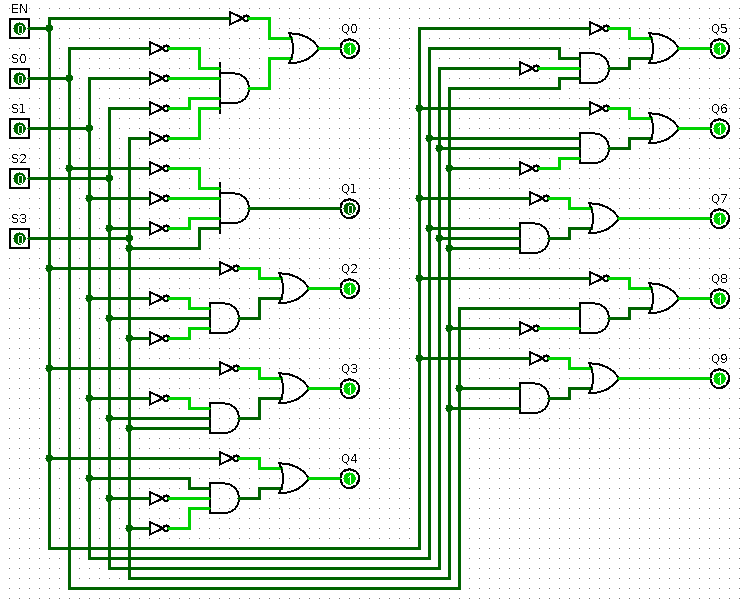
\includegraphics[width=1.0\textwidth]{imagens/romdec}
				\captionof{figure}{Circuito ROM Decoder}			
				EN: Bit de controlo de enable/disable\\
				S0-S3: Conjunto de 4 bits de entra que determina a escolha da ROM a ser utilizada\\
				Q0-Q9: Bit de controlo de saída com escolha de ROM \\
				\begin{table}[!ht]
					\centering
					\caption{Tabela de Seleção de ROM}
					\label{romd}
					\resizebox{0.7\textwidth}{!}{%
						\begin{tabular}{@{}|l|llll|llllllllll|@{}}
							\toprule
							\rowcolor[HTML]{BBDAFF} 
							& S3 & S2 & S1 & S0 & Q0 & Q1 & Q2 & Q3 & Q4 & Q5 & Q6 & Q7 & Q8 & Q9\\ \midrule
							0 & 0 & 0 & 0 & 0 & 1 & 0 & 0 & 0 & 0 & 0 & 0 & 0 & 0 & 0\\
							1 & 0 & 0 & 0 & 1 & 0 & 1 & 0 & 0 & 0 & 0 & 0 & 0 & 0 & 0\\
							2 & 0 & 0 & 1 & 0 & 0 & 0 & 1 & 0 & 0 & 0 & 0 & 0 & 0 & 0\\
							3 & 0 & 0 & 1 & 1 & 0 & 0 & 0 & 1 & 0 & 0 & 0 & 0 & 0 & 0\\
							4 & 0 & 1 & 0 & 0 & 0 & 0 & 0 & 0 & 1 & 0 & 0 & 0 & 0 & 0\\
							5 & 0 & 1 & 0 & 1 & 0 & 0 & 0 & 0 & 0 & 1 & 0 & 0 & 0 & 0\\
							6 & 0 & 1 & 1 & 0 & 0 & 0 & 0 & 0 & 0 & 0 & 1 & 0 & 0 & 0\\
							7 & 0 & 1 & 1 & 1 & 0 & 0 & 0 & 0 & 0 & 0 & 0 & 1 & 0 & 0\\
							8 & 1 & 0 & 0 & 0 & 0 & 0 & 0 & 0 & 0 & 0 & 0 & 0 & 1 & 0\\
							9 & 1 & 0 & 0 & 1 & 0 & 0 & 0 & 0 & 0 & 0 & 0 & 0 & 0 & 1\\ \bottomrule
						\end{tabular}
					}
				\end{table}\\
	\section{Enquadramento}
	O trabalho descrito neste relatório foi realizado recorrendo à linguagem de programação C, assim como os recursos disponibilizados na unidade curricular.\\
		\subsection{Motivação}
			A principal motivação para a realização deste trabalho, resulta da importância em criar e otimizar um sistema digital, assim como demonstrar os conhecimentos alcançados na disciplina de sistemas digitais.\\
		\subsection{Objectivos}
			Pretende-se através deste trabalho, criar um sistema de luzes como 	
			Em ultima analise o sistema digital é um sistema eletrónico onde os níveis de tensão elétrica são  mapeados como “0” e “1”.\\
			Na saída do circuito encontram-se ligados LEDs que estarão acesos ou apagados com “1” ou “0”, respetivamente.\\
	\section{Conclusões}
		A matriz de leds desenvolvida, para além de permitir os requisitos pedidos no enunciado do trabalho prático, permite também o uso de animações com leds mais complexas, mais padrões disponíveis e sendo modular torna-se mais escalável, entre outras funcionalidades.\\
		De frisar que devido à liberdade proporcionada para a construção dos circuitos, quer na sua forma de desenvolvimento quer na implementação permitiu desta forma aguçar a curiosidade para o uso de diversos componentes do simulador Logisim.\\
		Foi sem duvida um desafio interessante, mas que por limitação de tempo, deixa ainda uma larga margem para melhoramentos.\\
	\newpage
	\section{Bibliografia}
	\bibliographystyle{plain}
	\bibliography{./bibliotecas}

	\newpage
	\section{Anexos}
		Ficheiro "relatorio.pdf" e "ledmatrix.circ" compactado num ficheiro "trabalho.zip".\\\\
		Não existem quaisquer códigos ou listagens adicionais.\\					
\end{document}          
